% !TeX TS-program = xelatex
\documentclass{beamer}
\usetheme{Copenhagen}
\usepackage{fontspec, xunicode, xltxtra}
\usepackage{amsmath, amsfonts, amssymb}
\usepackage{hyperref}
\usepackage{mathptmx}
\usepackage{listings}
\usepackage{graphicx}
\usepackage{epstopdf}
\usepackage{subfigure}
\usepackage[english]{babel}
\usepackage{ulem}
\usepackage{tikz}
\usepackage{mathdots}
\usepackage{yhmath}
\usepackage{cancel}
\usepackage{color}
\usepackage{siunitx}
\usepackage{array}
\usepackage{multirow}
\usepackage{amssymb}
\usepackage{gensymb}
\usepackage{tabularx}
\usepackage{booktabs}
\usepackage{algorithm}
\usepackage{algpseudocode}
\usetikzlibrary{fadings}
\setmonofont{Courier New}
\newfontfamily{\monotype}{Consolas}

\lstset {
	basicstyle = \small\monotype,
	language = C++,
	tabsize = 2,
	frame = single,
	breaklines = true,
	breakindent = 1.1em,
	numbers=left,
	stringstyle=\monotype,
	numberstyle=\footnotesize\monotype,
	firstnumber=1,
	basewidth={0.5em, 0.4em},
}


\renewcommand{\algorithmicrequire}{\textbf{Input:}} 
\renewcommand{\algorithmicensure}{\textbf{Output:}}

\title{Computational Geometry: \\ Principles and Practices}
\institute{Nanjing University ICPC Training Team}
\author{Chen Shaoyuan}
\date{August 8, 2019}

%\renewcommand{\vec}{\mathbf}
\setlength{\parskip}{0.2cm}

\begin{document}
\begin{frame}
  \titlepage
\end{frame}

\begin{frame}{Guidelines in Solving Geometry Problems}
	\textbf{Rule 1: Prefer vectors to parameters in equations when representing geometric objects}
	
	 For example, use a point (point can be viewed as a vector from the origin) and a directional vector to represent a straight line, instead of using the slope $k$ and intercept $b$.
	 
	 \pause
    \begin{itemize}[<+->]
		\item Vectors have clearer geometric meanings than parameters;
		\item Vectors have predefined aggregate operations (vector addition/subtraction, scalar multiplication, inner/outer product); when processing parameters we operate on scalars.
		\item There is usually no degenerate case in vector-based representations.
	\end{itemize}
\end{frame}

\begin{frame}[fragile]{Guidelines in Solving Geometry Problems}
    Implementation trick: a short yet powerful vector class
    
\begin{lstlisting}
typedef double T;
typedef complex<T> pt, vec;
inline T operator , (pt a, pt b) // inner product
  { return real(a) * real(b) + imag(a) * imag(b); }
inline T operator * (pt a, pt b) // outer product
  { return real(a) * imag(b) - imag(a) * real(b); }
\end{lstlisting}

\pause

Pros: vector addition/subtraction and scalar multiplication (and their corresponding assignment operators) are provided by \lstinline|std::complex|. Also, we may use functions applicable to \lstinline|std::complex|, e.g., \lstinline|std::abs| to get the length of the vector.

Cons: accessing individual component is a bit tedious. You may use \lstinline|real| and \lstinline|imag| functions.
\end{frame}

\begin{frame}[fragile]{Guidelines in Solving Geometry Problems}
	\textbf{Rule 2: Use integer arithmetics whenever possible}
	\pause
	\begin{itemize}
	\item Integer arithmetics have no precision issue, which prevents you from falling into epsilon-tuning trap.
    \end{itemize}
   
    \pause
    
	\textbf{Rule 3: Think twice before tuning epsilon}
	\pause
	\begin{itemize}[<+->]
	\item Most computational geometry problems, especially those that the output can be written as a continuous function of its input, do not need an epsilon.
	\item Even though a problem indeed requires an epsilon, it is more often that other part of your code causes the Wrong Answer.
	\end{itemize}
\end{frame}

\begin{frame}{Triangle Partition}
The triangle partition method arises from computing the area of a polygon: partition the polygon into several directed triangles, and compute the sum of the signed areas of the triangles.
\begin{figure}
	\centering
	
	\tikzset{every picture/.style={line width=0.75pt}} %set default line width to 0.75pt        
	
	\begin{tikzpicture}[x=0.75pt,y=0.75pt,yscale=-1,xscale=1]
	%uncomment if require: \path (0,300); %set diagram left start at 0, and has height of 300
	
	%Shape: Polygon [id:ds28749328809073305] 
	\draw  [fill={rgb, 255:red, 248; green, 231; blue, 28 }  ,fill opacity=0.5 ][dash pattern={on 0.84pt off 2.51pt}] (340,80) -- (299.66,160.24) -- (370,110) -- cycle ;
	%Shape: Polygon [id:ds9037448619940351] 
	\draw  [fill={rgb, 255:red, 208; green, 2; blue, 27 }  ,fill opacity=0.5 ][dash pattern={on 0.84pt off 2.51pt}] (360,150) -- (299.66,160.24) -- (370,110) -- cycle ;
	%Shape: Axis 2D [id:dp1468555549941939] 
	\draw  (110,160.24) -- (210,160.24)(119.66,70) -- (119.66,170) (203,155.24) -- (210,160.24) -- (203,165.24) (114.66,77) -- (119.66,70) -- (124.66,77)  ;
	%Shape: Polygon [id:ds8067923362423097] 
	\draw  [fill={rgb, 255:red, 248; green, 231; blue, 28 }  ,fill opacity=1 ] (130,120) -- (160,80) -- (190,110) -- (180,150) -- (160,120) -- cycle ;
	%Shape: Axis 2D [id:dp7150899385539968] 
	\draw  (290,160.24) -- (390,160.24)(299.66,70) -- (299.66,170) (383,155.24) -- (390,160.24) -- (383,165.24) (294.66,77) -- (299.66,70) -- (304.66,77)  ;
	%Shape: Polygon [id:ds14454604468906362] 
	\draw  [fill={rgb, 255:red, 144; green, 19; blue, 254 }  ,fill opacity=0.5 ][dash pattern={on 0.84pt off 2.51pt}] (340,120) -- (299.66,160.24) -- (310,120) -- cycle ;
	%Shape: Polygon [id:ds7661747943559092] 
	\draw  [fill={rgb, 255:red, 184; green, 233; blue, 134 }  ,fill opacity=0.5 ][dash pattern={on 0.84pt off 2.51pt}] (360,150) -- (299.66,160.24) -- (340,120) -- cycle ;
	%Shape: Polygon [id:ds4844560849120194] 
	\draw  [fill={rgb, 255:red, 65; green, 117; blue, 5 }  ,fill opacity=0.5 ][dash pattern={on 0.84pt off 2.51pt}] (340,80) -- (299.66,160.24) -- (310,120) -- cycle ;
	%Right Arrow [id:dp22614230088020637] 
	\draw   (230,115) -- (254,115) -- (254,110) -- (270,120) -- (254,130) -- (254,125) -- (230,125) -- cycle ;
	%Straight Lines [id:da4201827162756411] 
	\draw    (340,120) -- (358.89,148.34) ;
	\draw [shift={(360,150)}, rotate = 236.31] [fill={rgb, 255:red, 0; green, 0; blue, 0 }  ][line width=0.75]  [draw opacity=0] (8.93,-4.29) -- (0,0) -- (8.93,4.29) -- cycle    ;
	
	%Straight Lines [id:da8374853484721989] 
	\draw    (360,150) -- (369.51,111.94) ;
	\draw [shift={(370,110)}, rotate = 464.04] [fill={rgb, 255:red, 0; green, 0; blue, 0 }  ][line width=0.75]  [draw opacity=0] (8.93,-4.29) -- (0,0) -- (8.93,4.29) -- cycle    ;
	
	%Straight Lines [id:da5970195351785434] 
	\draw    (370,110) -- (341.41,81.41) ;
	\draw [shift={(340,80)}, rotate = 405] [fill={rgb, 255:red, 0; green, 0; blue, 0 }  ][line width=0.75]  [draw opacity=0] (8.93,-4.29) -- (0,0) -- (8.93,4.29) -- cycle    ;
	
	%Straight Lines [id:da015721442741390534] 
	\draw    (340,80) -- (311.2,118.4) ;
	\draw [shift={(310,120)}, rotate = 306.87] [fill={rgb, 255:red, 0; green, 0; blue, 0 }  ][line width=0.75]  [draw opacity=0] (8.93,-4.29) -- (0,0) -- (8.93,4.29) -- cycle    ;
	
	%Straight Lines [id:da7932359089500032] 
	\draw    (310,120) -- (338,120) ;
	\draw [shift={(340,120)}, rotate = 180] [fill={rgb, 255:red, 0; green, 0; blue, 0 }  ][line width=0.75]  [draw opacity=0] (8.93,-4.29) -- (0,0) -- (8.93,4.29) -- cycle    ;
	
	\end{tikzpicture}
\end{figure}

\pause

This yields the shoelace formula (aka Gauss's area formula or surveyor's formula):
$$
S_P = \frac{1}{2}\left|\sum_{i = 0}^{n - 1} \vec{P}_i \times \vec{P}_{i+1}\right|
\quad (P_n = P_0)
$$
\end{frame}

\begin{frame}{Triangle Partition}
From the view of calculus, this method is derived from the Green's formula:
$$ \iint_{P} \left(\frac{\partial M}{\partial x} - \frac{\partial L}{\partial y}\right) dx dy = \oint_{\partial P} (L dx + M dy) $$
and thus it can be used to compute double integral over a polygon.
\end{frame}

\begin{frame}{Triangle Partition Method}{ICPC WF'13 J: Pollution Solution}
Find the area of the intersection of a polygon and a circle.
\begin{figure}
\centering
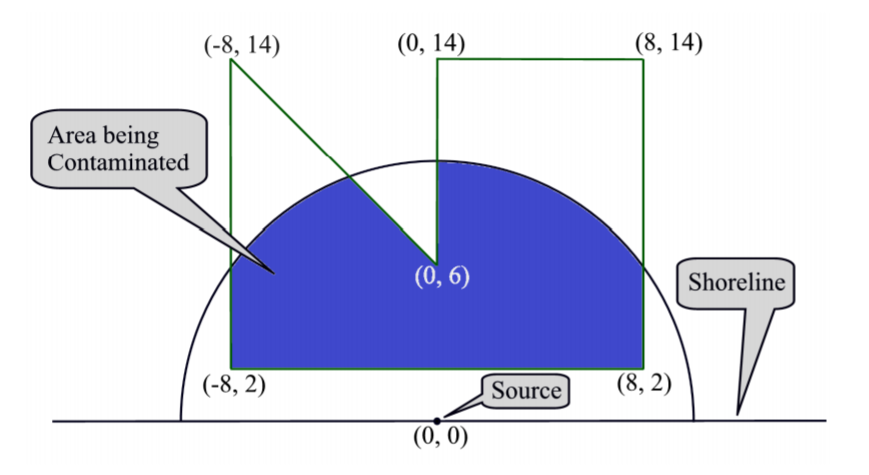
\includegraphics[width=8cm]{wf13j.png}
\end{figure}
\end{frame}

\begin{frame}{Triangular Partition}{ICPC WF'13 J: Pollution Solution}
Still partition the polygon into triangles. Compute the intersection of each triangle and the circle, and sum up their signed areas. (If the center of the circle is not origin, translate the coordinate system such that the center becomes the origin.)

\begin{figure}
	\centering


\tikzset{every picture/.style={line width=0.75pt}} %set default line width to 0.75pt        

\begin{tikzpicture}[x=0.75pt,y=0.75pt,yscale=-.7,xscale=.7]
%uncomment if require: \path (0,300); %set diagram left start at 0, and has height of 300

%Shape: Polygon [id:ds9604329650167358] 
\draw  [fill={rgb, 255:red, 248; green, 231; blue, 28 }  ,fill opacity=1 ] (320,60) -- (280,120) -- (320,140) -- cycle ;
%Shape: Circle [id:dp6702848289084407] 
\draw   (90,120) .. controls (90,92.39) and (112.39,70) .. (140,70) .. controls (167.61,70) and (190,92.39) .. (190,120) .. controls (190,147.61) and (167.61,170) .. (140,170) .. controls (112.39,170) and (90,147.61) .. (90,120) -- cycle ;
%Shape: Polygon [id:ds1210984443220029] 
\draw  [fill={rgb, 255:red, 248; green, 231; blue, 28 }  ,fill opacity=1 ] (120,90) -- (140,120) -- (180,130) -- cycle ;
%Shape: Circle [id:dp8334876120565433] 
\draw   (230,120) .. controls (230,92.39) and (252.39,70) .. (280,70) .. controls (307.61,70) and (330,92.39) .. (330,120) .. controls (330,147.61) and (307.61,170) .. (280,170) .. controls (252.39,170) and (230,147.61) .. (230,120) -- cycle ;
%Straight Lines [id:da9317657354345146] 
\draw    (280,120) -- (320,90) ;


%Shape: Polygon [id:ds16611928897149486] 
\draw  [fill={rgb, 255:red, 248; green, 231; blue, 28 }  ,fill opacity=1 ] (410,60) -- (420,120) -- (490,120) -- cycle ;
%Shape: Circle [id:dp39564098108764223] 
\draw   (370,120) .. controls (370,92.39) and (392.39,70) .. (420,70) .. controls (447.61,70) and (470,92.39) .. (470,120) .. controls (470,147.61) and (447.61,170) .. (420,170) .. controls (392.39,170) and (370,147.61) .. (370,120) -- cycle ;
%Shape: Polygon [id:ds397439665283462] 
\draw  [fill={rgb, 255:red, 248; green, 231; blue, 28 }  ,fill opacity=1 ] (600,60) -- (560,120) -- (640,120) -- cycle ;
%Shape: Circle [id:dp16904858813685153] 
\draw   (510,120) .. controls (510,92.39) and (532.39,70) .. (560,70) .. controls (587.61,70) and (610,92.39) .. (610,120) .. controls (610,147.61) and (587.61,170) .. (560,170) .. controls (532.39,170) and (510,147.61) .. (510,120) -- cycle ;
%Straight Lines [id:da42101863521839333] 
\draw    (420,120) -- (468.66,103.86) ;


%Straight Lines [id:da3077342337875624] 
\draw    (425.66,71.86) -- (420,120) ;

\end{tikzpicture}

\end{figure}

\pause

The first and the fourth can be computed directly. The second and third can be further partitioned to several triangles and compute separately.
\end{frame}

\begin{frame}{Triangle Partition}{Discover Vladivostok 2019. Division A Day 1: D. Zebra}
Define a point set $S$:
$$ S = \{(x, y): 2k \leq x \leq 2k + 1, k \in \mathbb{Z}\}. $$
Given a polygon $P$. Compute the area of the intersection of $P$ and $S$.

\pause

In this problem, we may partition the polygon into several trapezoids (instead of triangles), and compute their contributions separately.
\end{frame}

\begin{frame}[fragile]{Triangle Partition}
Exercise:

 \href{https://github.com/wcysai/Calabash/blob/master/ByteDance%20-%20Moscow%20Workshops%20ICPC%20Programming%20Camp%202019.%20Day%202%2C%20Div%20A./statements.pdf}{2019 MW-Bytedance Camp, Day 2, Divison A: D. Cross-section}
\end{frame}

\begin{frame}{Enumerating Local Optima}
There are many optimization problems in computational geometry. They usually requires to find a geometric object, possibly under some restrictions, such that some value is minimized/maximized.

In most cases the set of all feasible solutions is infinite. However, for these problems, the set of all local optima is often finite! This enables us to enumerate all local optima and pick the most optimal one.
\end{frame}

\begin{frame}{Enumerating Local Optima}{ICPC WF'17 A: Airport Construction}
Given a polygon (not necessarily convex), find a line segment entirely lies in the polygon, such that the length is maximized. (number of vertices does not exceed 200)

\begin{figure}
	\centering
	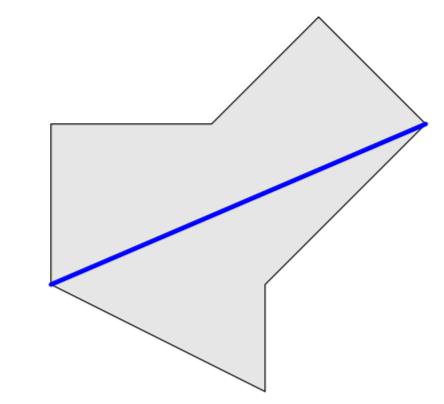
\includegraphics[width=4cm]{icpc17a.png}
\end{figure}
\end{frame}

\begin{frame}{Enumerating Local Optima}{ICPC WF'17 A: Airport Construction}
Observation: the optimal line segment must pass through at least two vertices of the polygon.

\pause

\begin{enumerate}[<+->]
	\item the endpoints of the line segment must be on the border of the polygon;
	\item if the line segment does not pass any vertex, translate the segment in some direction which will increase the length, until it touches a vertex of the polygon;
	\item if the line segment passes only one vertex, rotate the segment about the vertex clockwise or counterclockwise, depending on which one will increase the length of the segment.
\end{enumerate}
\end{frame}

\begin{frame}{Enumerating Local Optima}{ICPC WF'17 A: Airport Construction}
The algorithm
\begin{enumerate}
	\item for each vertex pair $A, B$:
	\begin{enumerate}
		\item check if segment $AB$ is entirely in the polygon;
		\item if so, extend the segment as far as possible.
	\end{enumerate}
	\item among all possible extended segments, pick the longest one.
\end{enumerate}

\pause

Checking if a segment is entirely in the polygon, and extending the segment can both be done in $O(n)$ time. The total time complexity is $O(n^3)$.
\end{frame}

\begin{frame}[fragile]{Enumerating Local Optima}
Exercise: 

NJUPC'19 H. Road Construction
\end{frame}

\begin{frame}{Sweep Line Algorithm}{An Introductory Example}

Given a set of orthogonal rectangles (sides parallel to axes). How to efficiently compute the area of their union?

\begin{figure}
\centering


\tikzset{every picture/.style={line width=0.75pt}} %set default line width to 0.75pt        

\begin{tikzpicture}[x=0.75pt,y=0.75pt,yscale=-1,xscale=1]
%uncomment if require: \path (0,300); %set diagram left start at 0, and has height of 300

%Shape: Rectangle [id:dp6693696661193478] 
\draw  [fill={rgb, 255:red, 248; green, 231; blue, 28 }  ,fill opacity=0.5 ] (40,30) -- (110,30) -- (110,70) -- (40,70) -- cycle ;
%Shape: Rectangle [id:dp3652386932643972] 
\draw  [fill={rgb, 255:red, 184; green, 233; blue, 134 }  ,fill opacity=0.5 ] (70,40) -- (100,40) -- (100,110) -- (70,110) -- cycle ;
%Shape: Rectangle [id:dp22825010751627506] 
\draw  [fill={rgb, 255:red, 189; green, 16; blue, 224 }  ,fill opacity=0.5 ] (90,10) -- (160,10) -- (160,50) -- (90,50) -- cycle ;
%Shape: Rectangle [id:dp2068836971585548] 
\draw  [fill={rgb, 255:red, 80; green, 227; blue, 194 }  ,fill opacity=0.5 ] (80,90) -- (150,90) -- (150,130) -- (80,130) -- cycle ;
%Shape: Rectangle [id:dp48363451619576137] 
\draw  [fill={rgb, 255:red, 245; green, 166; blue, 35 }  ,fill opacity=0.5 ] (130,40) -- (170,40) -- (170,110) -- (130,110) -- cycle ;

\end{tikzpicture}
\end{figure}

\pause

Imagine a line scans from left to right. Let $L(x_0)$ denote the total length of line $x=x_0$ clipped by the union of the rectangles. The total area is simply $\int_{-\infty}^{\infty} L(x) dx$.

\end{frame}

\begin{frame}{Sweep Line Algorithm}{An Introductory Example}
The algorithm:
\begin{itemize}
	\item Imagine a line scans from left to right.
	\item When the line enters a rectangle, add the vertically clipped segment into the set of intervals.
	\item When the line leaves a rectangle, delete the segment from the set of intervals.
	\item Before processing any of the above events, add to the answer the total length of the union of the intervals, times the distance of the scan line traveled since last event.
\end{itemize}

\pause

We need to maintain a set of intervals and the total length of their union. The naive solution gives $O(n^2)$ time. If we use data structures like segment tree or binary search tree, the total time is $O(n \log n)$.
\end{frame}

\begin{frame}{Sweep Line Algorithm}{An Introductory Example}
\begin{figure}
\centering
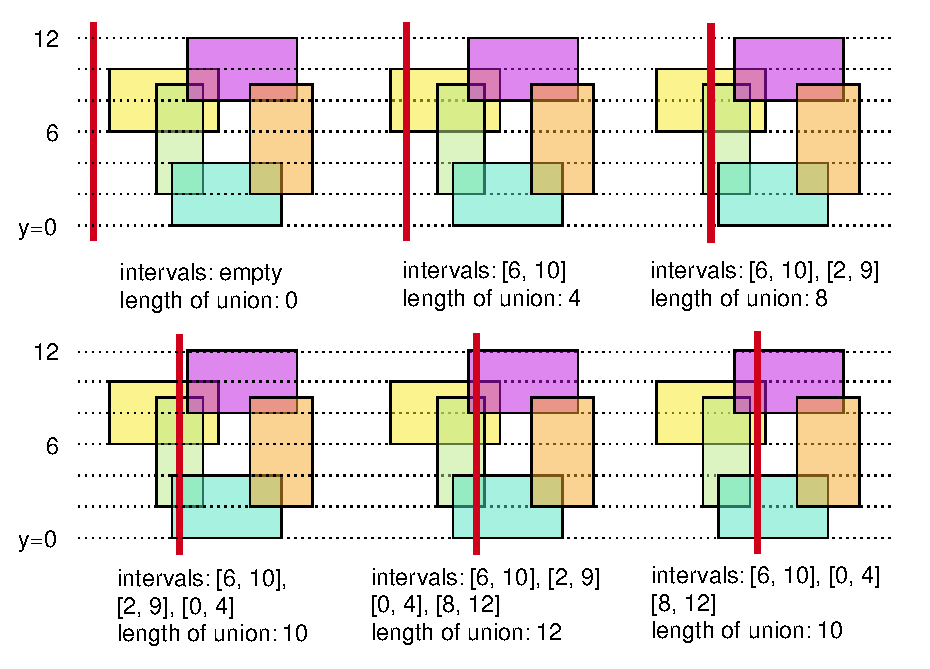
\includegraphics[width=10cm]{sweep.pdf}
\end{figure}
\end{frame}

\begin{frame}{Sweep Line Algorithm}{An Introductory Example}
Extension: given a set of orthogonal rectangles. You need to process several queries. Each query gives a point, and you need to answer the number of rectangles that contains the point.

\pause

Solution: sort the queries along with enter/leave events.

\pause

But, what if we need to process queries online? \pause We need to preserve the data structure after each operation. That's \textbf{persistence}! 

\pause

What if we need dynamically add/delete rectangles? \pause We need to edit the operation sequence as well as preserve the data structure after each operation. That's \textbf{retroactivity}!
\end{frame}

\begin{frame}{Data Structures}{Persistent Data Structure}
\textbf{Partial Persistence}

Support accessing all history versions, but only modifying the newest version.

\pause

Method: fat node

\lstinline|vector<pair<timestamp_t, value_t>> x;|

\begin{description}
	\item[Access] Binary search for timestamp;
	\item[Modify] \lstinline|x.push_back(timestamp++, new_value)|.
\end{description}

\pause

\textbf{Full Persistence}

Support accessing and modifying all history versions.

Method: path copying
\end{frame}

\begin{frame}{Data Structures}{Retroactive Data Structure}
\textbf{Partial Retroactivity}

Support modifying operation sequence and accessing the newest state of the data structure.

\begin{figure}
	\centering
	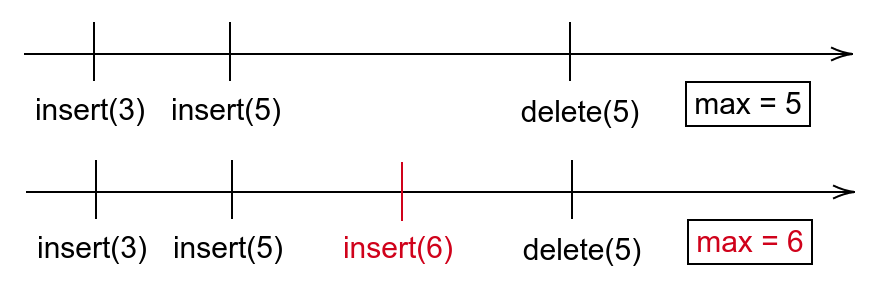
\includegraphics[width=7cm]{timeline.png}
\end{figure}

\textbf{Full Retroactivity}

Support modifying operation sequence and accessing the state of the data structure at any time point.

\end{frame}

\begin{frame}{Data Structures}{Decomposable Searching Problem}
A decomposable searching problem maintains a set $S$, which supports three operations:
\begin{itemize}
	\item Insert(S, x): add x to the set S;
	\item Delete(S, x): delete x from the set S;
	\item Query(S): query something in the set S;
\end{itemize}
and the Query operations can be obtained by combining Query results of disjoint subsets: Query(S + T) = f(Query(S), Query(T)).

\pause 

Using segment tree, we may easily make such data structure retroactive, with $O(\log n)$ overhead.

\end{frame}

\begin{frame}{Data Structures}{Decomposable Searching Problem}
\begin{figure}
	\centering
	
	
	\tikzset{every picture/.style={line width=0.75pt}} %set default line width to 0.75pt        
	
	\begin{tikzpicture}[x=0.75pt,y=0.75pt,yscale=-1,xscale=1]
	%uncomment if require: \path (0,300); %set diagram left start at 0, and has height of 300
	
	%Shape: Circle [id:dp40221891020232814] 
	\draw   (100,180) .. controls (100,174.48) and (104.48,170) .. (110,170) .. controls (115.52,170) and (120,174.48) .. (120,180) .. controls (120,185.52) and (115.52,190) .. (110,190) .. controls (104.48,190) and (100,185.52) .. (100,180) -- cycle ;
	%Shape: Circle [id:dp33577604295652774] 
	\draw   (140,180) .. controls (140,174.48) and (144.48,170) .. (150,170) .. controls (155.52,170) and (160,174.48) .. (160,180) .. controls (160,185.52) and (155.52,190) .. (150,190) .. controls (144.48,190) and (140,185.52) .. (140,180) -- cycle ;
	%Shape: Circle [id:dp5229953207344957] 
	\draw   (180,180) .. controls (180,174.48) and (184.48,170) .. (190,170) .. controls (195.52,170) and (200,174.48) .. (200,180) .. controls (200,185.52) and (195.52,190) .. (190,190) .. controls (184.48,190) and (180,185.52) .. (180,180) -- cycle ;
	%Shape: Circle [id:dp25699121649894097] 
	\draw   (220,180) .. controls (220,174.48) and (224.48,170) .. (230,170) .. controls (235.52,170) and (240,174.48) .. (240,180) .. controls (240,185.52) and (235.52,190) .. (230,190) .. controls (224.48,190) and (220,185.52) .. (220,180) -- cycle ;
	%Straight Lines [id:da8117362587070329] 
	\draw    (250,70) -- (170,90) ;
	
	
	%Straight Lines [id:da11286353627510581] 
	\draw    (170,100) -- (130,130) ;
	
	
	%Straight Lines [id:da3107583348759664] 
	\draw    (170,100) -- (210,130) ;
	
	
	%Shape: Circle [id:dp6401734620325106] 
	\draw  [fill={rgb, 255:red, 255; green, 255; blue, 255 }  ,fill opacity=1 ] (160,100) .. controls (160,94.48) and (164.48,90) .. (170,90) .. controls (175.52,90) and (180,94.48) .. (180,100) .. controls (180,105.52) and (175.52,110) .. (170,110) .. controls (164.48,110) and (160,105.52) .. (160,100) -- cycle ;
	%Straight Lines [id:da5886152916298026] 
	\draw    (130,140) -- (110,170) ;
	
	
	%Straight Lines [id:da09807922703191618] 
	\draw    (130,140) -- (150,170) ;
	
	
	%Shape: Circle [id:dp9524248842811434] 
	\draw  [fill={rgb, 255:red, 255; green, 255; blue, 255 }  ,fill opacity=1 ] (120,140) .. controls (120,134.48) and (124.48,130) .. (130,130) .. controls (135.52,130) and (140,134.48) .. (140,140) .. controls (140,145.52) and (135.52,150) .. (130,150) .. controls (124.48,150) and (120,145.52) .. (120,140) -- cycle ;
	%Straight Lines [id:da21037945260330004] 
	\draw    (210,140) -- (190,170) ;
	
	
	%Straight Lines [id:da39006409515695206] 
	\draw    (210,140) -- (230,170) ;
	
	
	%Shape: Circle [id:dp34065534716780466] 
	\draw  [fill={rgb, 255:red, 255; green, 255; blue, 255 }  ,fill opacity=1 ] (200,140) .. controls (200,134.48) and (204.48,130) .. (210,130) .. controls (215.52,130) and (220,134.48) .. (220,140) .. controls (220,145.52) and (215.52,150) .. (210,150) .. controls (204.48,150) and (200,145.52) .. (200,140) -- cycle ;
	%Shape: Circle [id:dp35073228190089956] 
	\draw   (260,180) .. controls (260,174.48) and (264.48,170) .. (270,170) .. controls (275.52,170) and (280,174.48) .. (280,180) .. controls (280,185.52) and (275.52,190) .. (270,190) .. controls (264.48,190) and (260,185.52) .. (260,180) -- cycle ;
	%Shape: Circle [id:dp5437661362151764] 
	\draw   (300,180) .. controls (300,174.48) and (304.48,170) .. (310,170) .. controls (315.52,170) and (320,174.48) .. (320,180) .. controls (320,185.52) and (315.52,190) .. (310,190) .. controls (304.48,190) and (300,185.52) .. (300,180) -- cycle ;
	%Shape: Circle [id:dp9923938722062762] 
	\draw   (340,180) .. controls (340,174.48) and (344.48,170) .. (350,170) .. controls (355.52,170) and (360,174.48) .. (360,180) .. controls (360,185.52) and (355.52,190) .. (350,190) .. controls (344.48,190) and (340,185.52) .. (340,180) -- cycle ;
	%Shape: Circle [id:dp8925746163699286] 
	\draw   (380,180) .. controls (380,174.48) and (384.48,170) .. (390,170) .. controls (395.52,170) and (400,174.48) .. (400,180) .. controls (400,185.52) and (395.52,190) .. (390,190) .. controls (384.48,190) and (380,185.52) .. (380,180) -- cycle ;
	%Straight Lines [id:da8190561290246585] 
	\draw    (330,100) -- (290,130) ;
	
	
	%Straight Lines [id:da48148385368575175] 
	\draw    (330,100) -- (370,130) ;
	
	
	%Shape: Circle [id:dp0015853245433787855] 
	\draw  [fill={rgb, 255:red, 255; green, 255; blue, 255 }  ,fill opacity=1 ] (320,100) .. controls (320,94.48) and (324.48,90) .. (330,90) .. controls (335.52,90) and (340,94.48) .. (340,100) .. controls (340,105.52) and (335.52,110) .. (330,110) .. controls (324.48,110) and (320,105.52) .. (320,100) -- cycle ;
	%Straight Lines [id:da6958977920058216] 
	\draw    (290,140) -- (270,170) ;
	
	
	%Straight Lines [id:da9855730897095563] 
	\draw    (290,140) -- (310,170) ;
	
	
	%Shape: Circle [id:dp8907250959572885] 
	\draw  [fill={rgb, 255:red, 255; green, 255; blue, 255 }  ,fill opacity=1 ] (280,140) .. controls (280,134.48) and (284.48,130) .. (290,130) .. controls (295.52,130) and (300,134.48) .. (300,140) .. controls (300,145.52) and (295.52,150) .. (290,150) .. controls (284.48,150) and (280,145.52) .. (280,140) -- cycle ;
	%Straight Lines [id:da7364191584309807] 
	\draw    (370,140) -- (350,170) ;
	
	
	%Straight Lines [id:da5412245774912621] 
	\draw    (370,140) -- (390,170) ;
	
	
	%Shape: Circle [id:dp05268934157596816] 
	\draw  [fill={rgb, 255:red, 255; green, 255; blue, 255 }  ,fill opacity=1 ] (360,140) .. controls (360,134.48) and (364.48,130) .. (370,130) .. controls (375.52,130) and (380,134.48) .. (380,140) .. controls (380,145.52) and (375.52,150) .. (370,150) .. controls (364.48,150) and (360,145.52) .. (360,140) -- cycle ;
	%Straight Lines [id:da6530965464009104] 
	\draw    (250,70) -- (330,90) ;
	
	
	%Shape: Circle [id:dp5238021079711781] 
	\draw  [fill={rgb, 255:red, 255; green, 255; blue, 255 }  ,fill opacity=1 ] (240,70) .. controls (240,64.48) and (244.48,60) .. (250,60) .. controls (255.52,60) and (260,64.48) .. (260,70) .. controls (260,75.52) and (255.52,80) .. (250,80) .. controls (244.48,80) and (240,75.52) .. (240,70) -- cycle ;
	%Straight Lines [id:da5285155640142385] 
	\draw [color={rgb, 255:red, 74; green, 144; blue, 226 }  ,draw opacity=1 ][line width=1.5]    (179,225) -- (359,225) ;
	\draw [shift={(359,225)}, rotate = 180] [color={rgb, 255:red, 74; green, 144; blue, 226 }  ,draw opacity=1 ][line width=1.5]    (0,6.71) -- (0,-6.71)   ;
	\draw [shift={(179,225)}, rotate = 180] [color={rgb, 255:red, 74; green, 144; blue, 226 }  ,draw opacity=1 ][line width=1.5]    (0,6.71) -- (0,-6.71)   ;
	%Straight Lines [id:da13790800874259257] 
	\draw [color={rgb, 255:red, 208; green, 2; blue, 27 }  ,draw opacity=1 ][line width=1.5]    (101,247) -- (319.44,247) ;
	\draw [shift={(319.44,247)}, rotate = 180] [color={rgb, 255:red, 208; green, 2; blue, 27 }  ,draw opacity=1 ][line width=1.5]    (0,6.71) -- (0,-6.71)   ;
	\draw [shift={(101,247)}, rotate = 180] [color={rgb, 255:red, 208; green, 2; blue, 27 }  ,draw opacity=1 ][line width=1.5]    (0,6.71) -- (0,-6.71)   ;
	
	% Text Node
	\draw (161.5,224) node [color={rgb, 255:red, 74; green, 144; blue, 226 }  ,opacity=1 ] [align=left] {A};
	% Text Node
	\draw (229.5,137) node [color={rgb, 255:red, 74; green, 144; blue, 226 }  ,opacity=1 ] [align=left] {A};
	% Text Node
	\draw (309.5,137) node [color={rgb, 255:red, 74; green, 144; blue, 226 }  ,opacity=1 ] [align=left] {A};
	% Text Node
	\draw (365.5,170) node [color={rgb, 255:red, 74; green, 144; blue, 226 }  ,opacity=1 ] [align=left] {A};
	% Text Node
	\draw (110,203) node  [align=left] {1};
	% Text Node
	\draw (151,202) node  [align=left] {2};
	% Text Node
	\draw (190,202) node  [align=left] {3};
	% Text Node
	\draw (231,202) node  [align=left] {4};
	% Text Node
	\draw (270,202) node  [align=left] {5};
	% Text Node
	\draw (309,202) node  [align=left] {6};
	% Text Node
	\draw (350,202) node  [align=left] {7};
	% Text Node
	\draw (390,202) node  [align=left] {8};
	% Text Node
	\draw (86.5,247) node [color={rgb, 255:red, 208; green, 2; blue, 27 }  ,opacity=1 ] [align=left] {B};
	% Text Node
	\draw (150.5,90) node [color={rgb, 255:red, 208; green, 2; blue, 27 }  ,opacity=1 ] [align=left] {B};
	% Text Node
	\draw (321.5,137) node [color={rgb, 255:red, 208; green, 2; blue, 27 }  ,opacity=1 ] [align=left] {B};
	
	
	\end{tikzpicture}
	
\end{figure}

\end{frame}

\begin{frame}{Sweep Line Algorithm}{ICPC WF'16 G: Oil}
Given a set of horizontal line segments, find a line that intersects maximum number of them. There are at most 2000 segments. No two segments intersect, not even at a point.
\begin{figure}
	\centering
	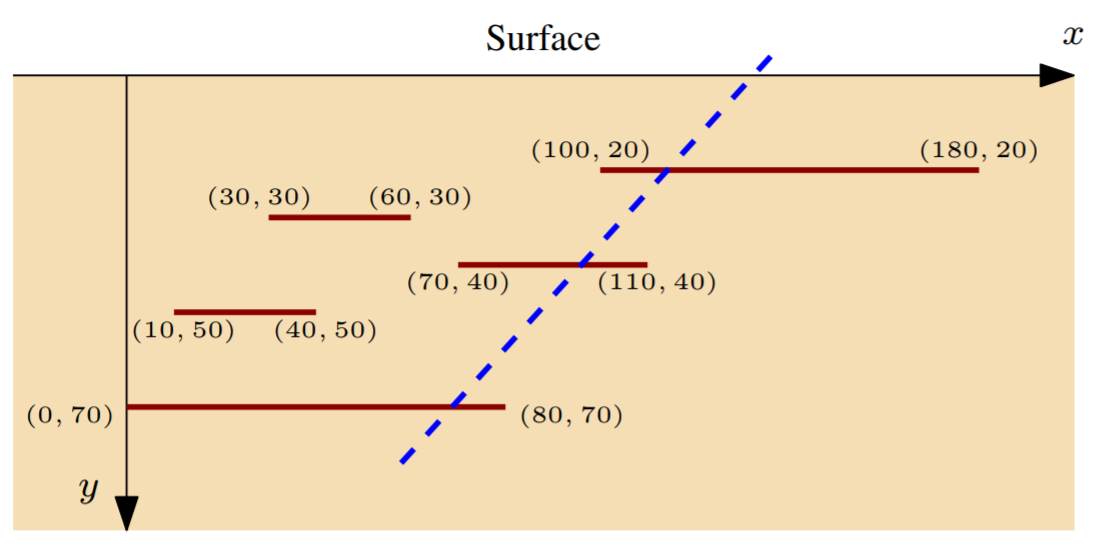
\includegraphics[width=10cm]{icpc16g.png}
\end{figure}
\end{frame}

\begin{frame}{Sweep Line Algorithm}{ICPC WF'16 G: Oil}
This is an optimization problem. We can use the \textbf{enumerating local optima} paradigm!

\pause

Not hard to prove that the optimal line passes through at least two end points of these line segments.

\pause

However, enumerating all such lines and counting the number of intersections for each of these lines take $O(n^3)$ time.

\pause

We may enumerate one end point. Consider a line passing this end point, and we rotate this line. During rotation, several \textit{enter} and \textit{leave} events occur, and we only have to maintain the number of intersections. Just sort all other points by their polar angles to the fixed end points. The total time complexity is thus reduced to $O(n^2 \log n)$.
\end{frame}

\begin{frame}{Sweep Line Algorithm}
Exercise: 

Determining whether any two line segments in a set of segments intersect, in $O(n \log n)$ time. 
\end{frame}

\begin{frame}{Overview}
Three rules on writing geometry problems:
\begin{enumerate}
	\item Prefer vectors to parameters in equations when representing geometric objects;
	\item Use integer arithmetics whenever possible;
	\item Think twice before tuning epsilon.
\end{enumerate}

Three algorithmic paradigms on solving geometry problems:
\begin{enumerate}
	\item Triangle/trapezoid partition;
	\item Enumerating local optima;
	\item (Rotational) sweep line.
\end{enumerate}
\end{frame}


\end{document}